\documentclass[letterpaper,10pt]{article}

\usepackage[margin=64pt]{geometry}
\usepackage{amsthm}
\usepackage{amsmath}
\usepackage{amssymb}
\usepackage{enumerate}
\usepackage{graphicx}
\usepackage{hyperref}
\usepackage{parskip}
\usepackage{pgfplots}
\usepackage{relsize}
\usepackage{tikz}

\usepgfplotslibrary{fillbetween}
\setcounter{secnumdepth}{0}
\allowdisplaybreaks[1]

\newcommand{\doubleu}[1]{\underline{\underline{#1}}}
\newcommand{\ddx}[1]{\frac{d}{dx} \bigg( #1 \bigg)}
\newcommand{\partiald}[2]{\frac{\partial #1}{\partial #2}}
\newcommand{\matrixpartiald}[2]{\dfrac{\partial #1}{\partial #2}}
\newcommand{\mathematica}[1]{Mathematica: \texttt{#1}}
\newcommand{\intbyparts}[7]{
	\begin{aligned}
		\text{Let}\   #1 &= #4      &      &\text{and}\    &   #2 &= #6 \\
		\Rightarrow \frac{d#1}{d#3} &= #5 \   &  &   &  \Rightarrow \frac{d#2}{d#3} &= #7
	\end{aligned}
	\\ \text{We know} \  \int #1 \, d#2 = #1#2 - \int #2 \, d#1 \\
	= {#4 \cdot #6} - \int {#6 \cdot #5} \, d#3
}

\begin{document}
	\noindent {\bf Rukmal Weerawarana (1337197)} \newline
	\noindent {\bf CFRM 460} \newline
	\noindent {\bf Homework 4 Solutions} \newline
	\noindent {\bf 2/5/16}
	\newline \hrule


	\section{Question 1}
		\subsection{Part (a)}
			\begin{gather*}
				\text{The assumptions of Fubini's theorum are as follows:} \\
				\iint_D f(x,y) \, dA < \infty
			\end{gather*}
		\subsection{Part (b)}
			\begin{gather*}
				\iint_D e^{y^2} \, dA \text{, where } D = \{(x,y): 0 \leq y \leq 1, 0 \leq x \leq y\} \\
				\text{The region D is as follows:}
			\end{gather*}
			{\centering
			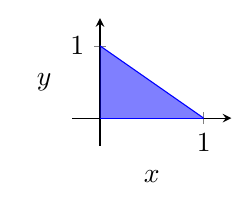
\begin{tikzpicture}
				\begin{axis} [
					axis lines = left,
					axis line style={shorten >=-10pt, shorten <=-10pt},
					xlabel = $x$,
					ylabel = $y$,
					ylabel style={rotate=-90},
					ytick={1},
					xtick={1},
					height=2.5cm
					]
					\addplot [name path=line, domain=1:0, color=blue] {1-x};
					\addplot [name path=axis, domain=1:0, color=blue] {0};
					\addplot [
					thick,
					color=blue,
					fill=blue,
					opacity=0.5
					]
					fill between[
					of=line and axis,
					soft clip={domain=0:1},
					];
				\end{axis}
			\end{tikzpicture}
			\par}
			\begin{gather*}
				\Rightarrow \iint_D e^{y^2} \, dA = \int_0^1\int_0^y e^{y^2} \, dxdy \\
				= \int_0^1 \left[ xe^{y^2} \right]_0^y \, dy = \int_0^1 ye^{y^2} \, dy = \left[ \frac{1}{2}e^{y^2} \right]_0^1 = \doubleu{\frac{e}{2} - \frac{1}{2}}
			\end{gather*}


	\section{Question 2}
		\subsection{Part (a)}
			\begin{gather*}
				\iint_D e^{\frac{x+y}{x-y}} \, dA \\
				\text{Changing variables using:} \\
				u = x + y \tag{1} \\
				v = x - y \tag{2} \\
				\text{Expressing $x$ and $y$ in terms of $u$ and $v$:} \\
				\text{(1)$+$(2)} \rightarrow x = \frac{u+v}{2} \\
				\text{(1)$-$(2)} \rightarrow y = \frac{u-v}{2} \\
				\text{Substituting these values of $x$ and $y$ in the initial equation:} \\
				e^{\frac{x+y}{x-y}} = \exp{\left[ \frac{x+y}{x-y} \right]} = \exp{ \left[ \frac{ \frac{u+v}{2} + \frac{u-v}{2} }{ \frac{u+v}{2} - \frac{u-v}{2} } \right]} = \exp{ \left[ \frac{ \frac{u+v+u-v}{2} }{ \frac{u+v-u+v}{2} } \right]} \\
				= \exp {\left[ \frac{ \frac{2u}{2} }{ \frac{2v}{2} } \right]} = \exp{\left[ \frac{u}{v} \right]} = e^{\frac{u}{v}} \\
				\text{Calculating the Jacobian for the change of variables:} \\
				\Rightarrow \text{D}(x(u,v), y(u,v)) =
				\begin{bmatrix}
					\matrixpartiald{x}{u} & \matrixpartiald{x}{v} \\
					\\
					\matrixpartiald{y}{u} & \matrixpartiald{y}{v}
				\end{bmatrix}
				=
				\begin{bmatrix}
					\dfrac{1}{2} & \dfrac{1}{2} \\
					\\
					\dfrac{1}{2} & -\dfrac{1}{2}
				\end{bmatrix} \\
				\text{Finding the determinant of the Jacobian:} \\
				\Rightarrow \det \left[ D(x(u,v), y(u,v)) \right] = \partiald{x}{u}\partiald{y}{v} - \partiald{x}{v}\partiald{y}{u} = \left( \frac{1}{2} \cdot -\frac{1}{2} \right) - \left( \frac{1}{2} \cdot \frac{1}{2} \right) = -\frac{1}{4} - \frac{1}{4} = -\frac{1}{2} \\
				\text{Applying the 2-dimensional change of variable formula:} \\
				\Rightarrow \iint_D e^{\frac{x+y}{x-y}} \, dA = \iint_S e^{\frac{u}{v}} \cdot \left[ \partiald{x}{u}\partiald{y}{v} - \partiald{x}{v}\partiald{y}{u} \right] \, dS = \doubleu{ \iint_S -\frac{1}{2} e^{\frac{u}{v}} \, dvdu }
			\end{gather*}

		\subsection{Part (b)}
			\begin{center}
			\begin{gather*}
				\text{Region D is bound by the following vertices on the $xy$ plane:} \\
				(x_1,y_1) = (1,0) \\
				(x_2,y_2) = (2,0) \\
				(x_3,y_3) = (0,-2) \\
				(x_4,y_4) = (0,-1) \\
				\text{Plotting Region D on the $xy$ plane:}
			\end{gather*}
			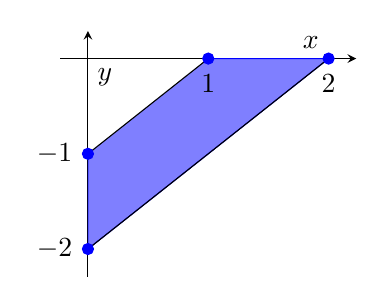
\begin{tikzpicture}
				\begin{axis} [
					axis lines = middle,
					axis line style={shorten >=-10pt, shorten <=-10pt},
					xlabel = $x$,
					ylabel = $y$,
					xtick = {1,2},
					ytick = {-1,-2},
					height=4cm
					]
					\addplot [color=blue, mark=*] coordinates {(1,0) (2,0) (0,-2) (0,-1)};
					\addplot [name path=line1, domain=0:1] {x-1};
					\addplot [name path=line2, domain=0:2] {x-2};
					\addplot [
					thick,
					color=blue,
					fill=blue,
					opacity=0.5
					]
					fill between[
					of=line1 and line2,
					soft clip={domain=0:2},
					];
				\end{axis}
			\end{tikzpicture}
			\begin{gather*}
				\text{Transforming the vertices of Region D from the $xy$ plane to the $uv$ plane using $u=x+y$ and $v=x-y$:} \\
				(x_1,y_1) = (1,0) \Rightarrow (u_1,v_1) = (1,1) \\
				(x_2,y_2) = (2,0) \Rightarrow (u_2,v_2) = (2,2) \\
				(x_3,y_3) = (0,-2) \Rightarrow (u_3,v_3) = (-2,2) \\
				(x_4,y_4) = (0,-1) \Rightarrow (u_4,v_4) = (-1,1) \\
				\therefore \, \text{Region S has vertices $(u_1,v_1), (u_2,v_2), (u_3,v_3), (u_4,v_4)$ on the $uv$ plane.} \\
				\text{Plotting Region S on the $uv$ plane:}
			\end{gather*}
			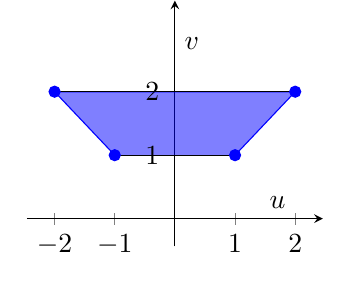
\begin{tikzpicture}
				\begin{axis} [
					axis lines = middle,
					axis line style={shorten >=-10pt, shorten <=-10pt},
					xlabel = $u$,
					ylabel = $v$,
					ytick = {1,2},
					ymax = 3,
					height=4cm
					]
					\addplot [color=blue, mark=*] coordinates {(1,1) (2,2) (-2,2) (-1,1)};
					\addplot [name path=line1, domain=-2:2] {2};
					\addplot [name path=line2, domain=-1:1] {1};
					\addplot [name path=line3, domain=-1:1] {0};
					\addplot [
					thick,
					color=blue,
					fill=blue,
					opacity=0.5
					]
					fill between[
					of=line1 and line2,
					soft clip={domain=-2:2},
					];
				\end{axis}
			\end{tikzpicture}
			\end{center}

		\subsection{Part (c)}
			\begin{gather*}
				\iint_S -\frac{1}{2} e^{\frac{u}{v}} \, dvdu \\
				\text{Using the vertices of Region S from Part (b), Region S can be defined as follows:} \\
				S = \{ (u,v): -v \leq u \leq v, 1 \leq v \leq 2 \} \\
				\Rightarrow \iint_S -\frac{1}{2} e^{\frac{u}{v}} \, dvdu = \int_1^2\int_{-v}^v -\frac{1}{2} e^{\frac{u}{v}} \, dudv = \int_1^2 \left[ -\frac{v}{2} e^{\frac{u}{v}} \right]_{-v}^{v} \, dv = \int_1^2 \left( -\frac{v}{2}e - \left( -\frac{v}{2} e^{-1} \right) \right)  dv \\
				\int_1^2 \frac{v}{2} \left( \frac{1}{e} - e \right) dv = \left[ \frac{v^2}{4} \left( \frac{1}{e} - e \right) \right]_1^2 = \left( \frac{1}{e} - e \right) - \frac{1}{4} \left( \frac{1}{e} - e \right) = \doubleu{ \frac{3}{4} \left( \frac{1}{e} - e \right) }
			\end{gather*}


	\section{Question 3}
	 	\begin{gather*}
			\text{Recall, the Black-Scholes formula for the price of a European call option is as follows:} \\
			C(\cdot) = Se^{-q(T-t)} \Phi(d_+) - Ke^{-r(T-t)} \Phi(d_-) \\
			\text{Also, recall the Greeks $\Delta$ \& $\Gamma$, and how they are related to $C(\cdot)$:} \\
			\text{Delta, } \Delta (S) = \partiald{C(S)}{S} \\
			\text{Gamma, } \Gamma (S) = \partiald{^2C(S)}{S^2} \\
			\text{The taylor polynomial for a function $f(x)$ of order $n$ about a point $a$ is:} \\
			P_n(x) = f(a) + (x-a) f'(a) + \frac{(x-a)^2}{2}f''(a) + \dotsb + \frac{(x-a)^n}{n!}f^{(n)}(a) = \mathlarger{\mathlarger{\sum}}_{k=0}^n \frac{(x-a)^k}{k!} f^{(k)}(a) \\
			\Rightarrow \, \text{By using the information above, and treating $C(\cdot)$ as a function of a single variable S,} \\
			\text{the second-order taylor polynomial around point $S_0$ for $C(S)$ is as follows:} \\
			P_2(x) = f(a) + (x-a)f'(a) + \frac{(x-a)^2}{2}f''(a) \\
			\Rightarrow P_2(S) = C(S_0) + (S-S_0)\partiald{}{S}(C(S_0)) + \frac{(S-S_0)^2}{2}\partiald{^2}{S^2}(C(S_0)) \\
			= C(S_0) + (S-S_0)\Delta(S_0) + \left(\frac{S^2}{2} - S_0S + \frac{S_0^2}{2}\right)\Gamma(S_0) = C(S_0) + S \Delta(S_0) -  S_0 \Delta(S_0)+ \frac{\Gamma}{2}S^2 - S_0\Gamma(S_0)S + \frac{\Gamma(S_0)S_0^2}{2} \\
			\therefore P_2(S) = \doubleu{ \frac{\Gamma(S_0)}{2} S^2 + \left( \Delta(S_0) - S_0 \Gamma(S_0) \right) S + \left( C(S_0) - S_0\Delta(S_0) + \frac{S_0^2\Gamma(S_0)}{2} \right) }
		\end{gather*}


	\section{Question 4}
		\subsection{Part (a)}
			\begin{center}
			\begin{gather*}
				\iint_D \sqrt{x^2+y^2} \, dxdy \\
				\text{Where } D = \{ (x,y) : 1 \leq x^2+y^2 \leq 9, y \geq 0 \} \\
				\text{Plotting Region D on the $xy$ plane:}
			\end{gather*}
			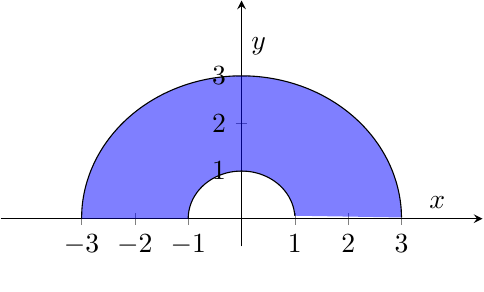
\begin{tikzpicture}
				\begin{axis} [
					axis lines = middle,
					axis line style={shorten >=-10pt, shorten <=-10pt},
					xlabel = $x$,
					ylabel = $y$,
					xtick = {-3,-2,-1,0,1,2,3},
					ytick = {0,1,2,3},
					xmin = -4,
					xmax = 4,
					ymax = 4,
					height=4cm,
					width=7cm
					]
					\addplot [name path=line1, domain=-3:3, samples=1000] {sqrt(9-x^2)};
					\addplot [name path=line2, domain=-1:1, samples=1000] {sqrt(1-x^2)};
					\addplot [
					thick,
					color=blue,
					fill=blue,
					opacity=0.5
					]
					fill between[
					of=line1 and line2,
					soft clip={domain=-3:4},
					];
				\end{axis}
			\end{tikzpicture}
			\begin{gather*}
				\text{Using the change of variable formula to convert the integral to polar coordinates using:} \\
				x = r\cos{(\theta)} \tag{1} \\
				y = r\sin{(\theta)} \tag{2} \\
				\text{Squaring both (1) and (2) results in the following:} \\
				\text{(1)} \cdot \text{(1)} \rightarrow x^2 = r^2 \cos^2{(\theta)} \tag{3} \\
				\text{(2)} \cdot \text{(2)} \rightarrow y^2 = r^2 \sin^2{(\theta)} \tag{4} \\
				\text{(3)} + \text{(4)} \rightarrow x^2 + y^2 = r^2 \sin^2{(\theta)} + r^2 \cos^2{(\theta)} = r^2(\cos^2{(\theta)} + \sin^2{(\theta)}) \\
				\text{But, we know $\cos^2{(\theta)} + \sin^2{(\theta)} = 1$. Thus:} \\
				r = \sqrt{x^2 + y^2} \\
				\text{To find an expression for $\theta$ in terms of $x$ and $y$, consider the following:} \\
				\frac{\text(2)}{\text{(1)}} \rightarrow \frac{y}{x} = \frac{\sin{(\theta)}}{\cos{(\theta)}} \\
				\text{But, we know $\frac{\sin{(\theta)}}{\cos{(\theta)}} = \tan{(\theta)}$. Thus:} \\
				\theta = \arctan{\left( \frac{y}{x} \right)} \\
				\\
				\text{Using this, the cartesian region can be converted to polar as follows:} \\
				1 \leq x^2+y^2 \leq 9 \Rightarrow 1 \leq \sqrt{x^2+y^2} \leq 3 \Rightarrow 1 \leq \theta \leq 3 \\
				y \geq 0 \Rightarrow \theta = \arctan{(0)} \Rightarrow \theta = 0 \text{ or } \theta = \pi \\
				\text{Let the cartesian Region D be equivalent to polar Region S. Thus,} \\
				D = \{ (x,y): 1 \leq x^2 + y^2 \leq 9, y \geq 0 \} \leftrightarrow S = \{ (r,\theta): 1 \leq r \leq 3, 0 \leq \theta \leq \pi \} \\
				\text{Plotting Region S on the $r\theta$ plane:}
			\end{gather*}
			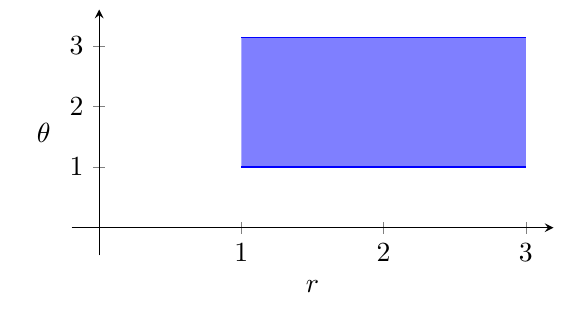
\begin{tikzpicture}
				\begin{axis} [
					axis lines = left,
					axis line style={shorten >=-10pt, shorten <=-10pt},
					xlabel = $r$,
					ylabel = $\theta$,
					xtick = {1,2,3},
					ytick = {1,2,3},
					xmin = 0,
					ymin = 0,
					ylabel style={rotate=-90},
					height=4cm,
					width=7cm
					]
					\addplot [name path=line1, color=blue, domain=1:3] {pi};
					\addplot [name path=line2, color=blue, domain=1:3] {1};
					\addplot [
					thick,
					color=blue,
					fill=blue,
					opacity=0.5
					]
					fill between[
					of=line1 and line2,
					soft clip={domain=1:3},
					];
				\end{axis}
			\end{tikzpicture}
			\begin{gather*}
				\text{Applying the change of variables to polar coordinates formula to the original integral:} \\
				\iint_D \sqrt{x^2+y^2} \, dxdy = \iint_S r \sqrt{(r\cos(\theta))^2 + (r \sin (\theta))^2} \, drd\theta \\
				= \iint_S r \sqrt{r^2(\cos^2(\theta) + \sin^2(\theta))} \, drd\theta = \iint_S r \sqrt{r^2} \, drd\theta = \iint_S r^2 \, drd\theta \\
				\text{Recall, } S = \{ (r, \theta): 1 \leq r \leq 3, 0 \leq \theta \leq \pi \} \\
				\Rightarrow \iint_S r^2 \, drd\theta = \int_0^\pi \int_1^3 r^2 \, drd\theta \\
				= \int_0^\pi \left[ \frac{r^3}{3} \right]^3_1 d\theta = \int_0^\pi \left( \frac{27}{3} - \frac{1}{3} \right) d\theta = \int_0^\pi \frac{26}{3} \, d\theta = \left[ \frac{26}{3}\theta \right]_0^\pi = \doubleu{\frac{26\pi}{3}}
			\end{gather*}
			\end{center}

		\subsection{Part (b)}
			\begin{gather*}
				\iint_D \sin(\sqrt{x^2 + y^2}) \, dxdy \\
				\text{Where } D = \{ (x,y): \pi^2 \leq x^2+y^2 \leq 4\pi^2 \} \\
				\text{Converting to polar coordinates using the following from Part (a):} \\
				r = \sqrt{x^2+y^2} \\
				\theta = \arctan \left( \frac{y}{x} \right) \\
				\text{Finding the new bounds for $r$:} \\
				\pi^2 \leq x^2 + y^2 \leq 4\pi^2 \Rightarrow \pi^2 \leq x^2+y^2 \leq (2\pi)^2 \Rightarrow \pi \leq \sqrt{x^2 + y^2} \leq 2\pi \Rightarrow \pi \leq r \leq 2\pi \\
				\text{As there are no restrictions on the domain of the $y$ variable:} \\
				0 \leq \theta \leq 2\pi \\
				\text{Let cartesian Region D be equivalent to polar Region S. Thus:} \\
				D = \{ (x,y): \pi^2 \leq x^2 + y^2 \leq 4\pi^2 \} \leftrightarrow S = \{ (r,\theta): \pi \leq r \leq 2\pi, 0 \leq \theta \leq 2\pi \} \\
				\\
				\text{Applying the change of variables to polar coordinates formaul to the original integral:} \\
				\iint_D \sin(\sqrt{x^2+y^2)} \, dxdy = \iint_S r \sin (\sqrt{(r\cos(\theta))^2+(r\sin(\theta))^2} \, drd\theta = \iint_S r\sin(r) \, drd\theta \\
				\text{Recall, } S = \{ (r, \theta): \pi \leq r \leq 2\pi, 0 \leq \theta \leq 2\pi \} \\
				\Rightarrow \iint_S r\sin(r) \, drd\theta = \int_0^{2\pi} \int_\pi^{2\pi} r \sin(r) \, drd\theta \\
				\\
				\text{Consider the inner integral, $\int r\sin(r) \, dr$. Applying integration by parts:} \\
				\intbyparts{u}{v}{r}{r}{1}{-\cos(r)}{\sin(r)} \\
				= - (-\sin(r)) - r\cos(r) = \sin(r) - r\cos(r) \\
				\\
				\text{Substituting this back into the original integral:} \\
				\Rightarrow \int_0^{2\pi} \int_\pi^{2\pi} r \sin(r) \, drd\theta = \int_0^{2\pi} \left[ \sin(r) - r\cos(r) \right]_\pi^{2\pi} d\theta = \int_0^{2\pi} \left( (\sin(2\pi) - 2\pi\cos(2\pi)) - (\sin(\pi) - \pi\cos(\pi)) \right) d\theta \\
				= \int_0^{2\pi} \left( (0 - 2\pi) - (0 - \pi(-1)) \right) d\theta = \int_0^{2\pi} \left( -2\pi - \pi \right) d\theta = \int_0^{2\pi} -3\pi \, d\theta \\
				= \left[ -3\pi\theta \right]_0^{2\pi} = (-3\pi \cdot 2\pi) - (-3\pi \cdot 0) = \doubleu{-6\pi^2}
			\end{gather*}


	\section{Question 5}
		\begin{gather*}
			f(x) = \frac{1}{1+x} \\
			\Rightarrow f'(x) = \frac{-1}{(1+x)^2}, f''(x) = \frac{2}{(1+x)^3}, f'''(x) = \frac{-6}{(1+x)^4}, \dotsc , f^{(k)}(x) = \frac{(-1)^k \cdot k!}{(1+x)^{(k+1)}} \\
			\text{The Taylor series expansion of a function $f(x)$ about a point $a$ is:} \\
			T(x) = \mathlarger{\mathlarger{\sum}}_{k=0}^\infty a_k (x-a)^k \\
			\text{Where the power series coefficients, } a_k = \frac{f^{(k)}(a)}{k!} \\
			\text{Thus, the Taylor series expansion of $f(x)$ about the point $a=0$ is:} \\
			T(x) = \mathlarger{\mathlarger{\sum}}_{k=0}^\infty a_k (x-a)^k = \mathlarger{\mathlarger{\sum}}_{k=0}^\infty \frac{(-1)^k \cdot k! \cdot (x-a)^k}{k! \cdot (1+a)^{(k+1)}} = \mathlarger{\mathlarger{\sum}}_{k=0}^\infty \frac{(-1)^k \cdot x^k}{1^{(k+1)}} = \mathlarger{\mathlarger{\sum}}_{k=0}^\infty (-x)^k \\
			\therefore T(x) = \mathlarger{\mathlarger{\sum}}_{k=0}^\infty (-x)^k \\
			\\
			\text{The radius of convergence, $R$ can be determined as follows:} \\
			R = \frac{1}{\lim_{k \rightarrow \infty} |a_k|^{1/k}} \\
			\Rightarrow \lim_{k \rightarrow \infty} |a_k|^{1/k} = \lim_{k \rightarrow \infty} \left| \frac{(-1)^k \cdot k!}{(1+a)^{(k+1)} \cdot k!} \right|^{1/k} = \lim_{k \rightarrow \infty} \left| \frac{(-1)^k}{1^{(k+1)}} \right|^{1/k} = \lim_{k \rightarrow \infty} \left| (-1)^k \right|^{1/k} \\
			= \lim_{k \rightarrow \infty} \left| (-1)^{k \cdot (1/k)} \right| = \lim_{k \rightarrow \infty} \left| (-1) \right| = |-1| \\
			\Rightarrow \lim_{k \rightarrow \infty} |a_k|^{1/k} = 1 \\
			\therefore \, \text{Radius of convergence, } R = \frac{1}{\lim_{k \rightarrow \infty} |a_k|^{1/k}} = \frac{1}{1} = 1 \\
			\\
			T(x) = f(x) = \frac{1}{1+x} \text{ when there is an $r$ such that $0<r<R$ and} \\
			\lim_{k \rightarrow \infty} \left[ \frac{r^k}{k!} \max_{z \in [a-r,a+r]} \left|f^{(k)}(z)\right| \right] = 0
			\Rightarrow \lim_{k \rightarrow \infty} \left[ \frac{r^k}{k!} \max_{z \in [-r,r]} \left|\frac{(-1)^{k} \cdot k!}{(1+z)^{(k+1)}}\right| \right] = 0 \\
			\text{Thus, to maximize the function $f^(k)(z)$, the denominator must be minimized (i.e. set to the lower bound of $z$):} \\
			\lim_{k \rightarrow \infty} \left[ \frac{r^k}{k!} \max_{z \in [-r,r]} \left|\frac{(-1)^{k} \cdot k!}{(1+z)^{(k+1)}}\right| \right] = \lim_{k \rightarrow \infty} \left[ \frac{r^k}{k!} \cdot \left|\frac{(-1)^{k} \cdot k!}{(1-r)^{(k+1)}}\right| \right] = \lim_{k \rightarrow \infty} \left[ r^k \cdot \frac{1}{(1-r)(1-r)^k} \cdot |(-1)|^k \right] \\
			\Rightarrow \lim_{k \rightarrow \infty} \left[ \left( \frac{r}{1-r} \right)^k \cdot \frac{1}{1-r} \right] = 0 \\
			\text{For the above to be true, $\frac{r}{1-r} < 1$} \\
			\Rightarrow \frac{r}{1-r} < 1 \Rightarrow r < 1-r \Rightarrow 2r < 1 \Rightarrow r < \frac{1}{2} \\
			\therefore T(x) = f(x) = \frac{1}{1+x} \text{ for } |x| < \frac{1}{2}
		\end{gather*}


	\section{Question 6}
		\begin{gather*}
			r_t = \log \left( \frac{P_t}{P_{t-1}} \right)
			\text{As we are dealing with small values of $R_t$, the following can be stated:} \\
			R_t = 0.01 \Rightarrow \frac{P_t-P_{t-1}}{P_{t-1}} = 0.01 \\
			P_t - P_{t-1} = 0.01 P_{t-1} \Rightarrow P_t = 1.01P_{t-1} \\
			\text{Finding the first term of the taylor series expansion of $r_t$:} \\
			P_1(P_t) = \log \left( \frac{P_t}{P_{t-1}} \right) + \frac{(P_t-a)^k}{k!}f^{(k)}(P_t) = \log \left( \frac{P_t}{P_{t-1}} \right) + (P_t-a)\left( \frac{P_{t-1}-P_t}{P_tP_{t-1}} \right) \\
			\text{But $a$ is very small, so $P_t-a \approx P_t$:} \\
			\Rightarrow r_t \approx \log \left( \frac{P_t}{P_{t-1}} \right) + \frac{P_t - P_{t-1}}{P_{t-1}} \\
			\text{Recall, $P_t \approx 0.01P_{t-1} \Rightarrow log \left( \frac{P_t}{P_{t-1}} \right) \approx 0$} \\
			\therefore r_t \approx \frac{P_t-P_{t-1}}{P_{t-1}} = R_t \text{ for small values of $R_t$}
		\end{gather*}
\end{document}
